% Filename: history@camecc_lic.tex
% This code is part of 'Cursos CAMECC: Introducao ao LaTeX para o Curso 29 - Licenciatura em Matematica'
% 
% Description: This file correspond to the short history of technology around LaTeX using in the course.
% 
% Created: 07.06.12 11:30:49 AM
% Last Change: 07.06.12 11:30:53 AM
% 
% Authors:
% - Raniere Silva, r.gaia.cs@gmail.com
% 
% Organization: CAMECC - Centro Academico dos Estudantes do IMECC
% 
% Copyright (c) 2012, Raniere Silva. All rights reserved.
% 
% This work is licensed under the Creative Commons Attribution-ShareAlike 3.0 Unported License. To view a copy of this license, visit http://creativecommons.org/licenses/by-sa/3.0/ or send a letter to Creative Commons, 444 Castro Street, Suite 900, Mountain View, California, 94041, USA.
%
% This work is distributed in the hope that it will be useful, but WITHOUT ANY WARRANTY; without even the implied warranty of MERCHANTABILITY or FITNESS FOR A PARTICULAR PURPOSE.
%
\chapter{Hist\'{o}ria} \label{sch:history}
Podemos dizer que a hist\'{o}ria da computa\c{c}\~{a}o moderna tem in\'{i}cio com a cria\c{c}\~{a}o do ENIAC (Electronic Numerical Integrator and Computer), o primeiro computador digital eletr\^{o}nico de grande escala, criado em fevereiro de 1946 pelos cientistas norte-americanos John Eckert e John Mauchly, da Electronic Control Company.\nocite{Wikipedia:PT:ENIAC}

Por muitos anos o uso de computadores ficou restrito a grandes empresas e universidades como AT\&T Bell Labs, General Electric, Massachusetts Institute of Technology entre outros. Em 1969 foi lan\c{c}ado o sistema operacional UNIX que rapidamente passou a ser utilizado pela maioria dos usu\'{a}rios da \'{e}poca.\nocite{Wikipedia:EN:UNIX}

Nos anos 70 ocorreu uma grande mudan\c{c}a nas t\'{e}cnicas de produ\c{c}\~{a}o de livros e similares. Em 1977, Donald Knuth lan\c{c}ou a segunda edi\c{c}\~{a}o do segundo volume de sua obra ``The Art of Computer Programming'' e n\~{a}o gostou do resultado (na primeira edi\c{c}\~{a}o havia sido utilizada uma t\'{e}cnica de impress\~{a}o diferente). Por volta desse ano, Knuth viu pela primeira vez o resultado de um sistema tipogr\'{a}fico digital de alta qualidade e ficou interessado pelo mesmo. Motivado pelo ``problema'' com o seu livro ele acabou desenvolvendo o seu pr\'{o}prio sistema tipogr\'{a}fico, o TeX, que foi lan\c{c}ado em 1978.\nocite{Wikipedia:EN:TeX}

Usar o TeX n\~{a}o era f\'{a}cil. Em 1985, Leslie Lamport lan\c{c}a o LaTeX, uma linguagem de marca\c{c}\~{a} e preparativo do sistema para o TeX, facilitando a utiliza\c{c}\~{a}o do TeX.\nocite{Wikipedia:EN:LaTeX}

Os primeiros computadores pessoais, como o Apple I, surgem nos anos 70. E nos anos 80 os computadores come\c{c}am a invadir escrit\'{o}rios e depois lares, sendo que nessa d\'{e}cada s\~{a}o lan\c{c}ados o IBM Personal Computer (IBM PC), Lisa, Macintosh e v\'{a}rios clones (principalmente do IBM PC).

Em 1985, uma pequena \textit{start-up} chamada Microsoft lan\c{c}a seu sistema operacional, Windows, e seu processador de texto, Word, que possuia uma vers\~{a}o para Macintosh e foi um dos primeiros a possuir funcionalidades verdadeiramente WYSIWYG\footnote{Acr\^{o}nimo da express\~{a}o em ingl\^{e}s ``What You See Is What You Get'', cuja tradu\c{c}\~{a}o remete a algo como ``O que voc\^{e} v\^{e} \'{e} o que voc\^{e} obtem''.}. Por ser WYSIWYG,  utilizar o Word ou algum de seus concorrentes n\~{a}o exigia nenhum conhecimento pr\'{e}vio e isso acabou ofuscando o LaTeX.\footnote{\'{E} importante destacar que, tipicamente, os usu\'{a}rios do LaTeX (ou TeX) e do Word (ou concorr\^{e}ntes) possuem necessidades bastante diferentes.}

Com os computadores pessoais a Microsoft acabou adquirindo grande parte do mercado de sistemas operacionais para o seu produto, o Windows, por este ser compat\'{i}vel com os clones do IBM PC e possuir interface gr\'{a}fica.\footnote{Nessa \'{e}poca a Apple ainda era uma \textit{start-up} quando comparada a seus concorrentes como, por exemplo, a IBM e ocorria a \textit{UNIX wars} (ver detalhes em \url{http://en.wikipedia.org/wiki/Unix_wars}).} Desde que o Windows passou a ser o sistema operacional dominante\footnote{Ao menos no ramo de computadores pessoais.} a Microsoft violou v\'{a}rias leis antitruste para promover outros de seus produtos como seu pacote de escrit\'{o}rio, Microsoft Office, que inclue o Word, seu navegador de internet, Internet Explorer, e outros.

\begin{figure}[htb]
    \begin{center}
        % Filename: history_timeline1@latex_with_vim.tex
% This code is part of LaTeX with Vim.
% 
% Description: TikZ for teachers is free book about TikZ and Sage.
% 
% Created: 30.03.12 07:55:25 PM
% Last Change: 30.03.12 07:56:41 PM
% 
% Author: Raniere Gaia Costa da Silva, r.gaia.cs@gmail.com
% Organization:  
% 
% Copyright (c) 2010, 2011, 2012, Raniere Gaia Costa da Silva. All rights 
% reserved.
% 
% This file is license under the terms of a Creative Commons Attribution 
% 3.0 Unported License, or (at your option) any later version. More details
% at <http://creativecommons.org/licenses/by/3.0/>.
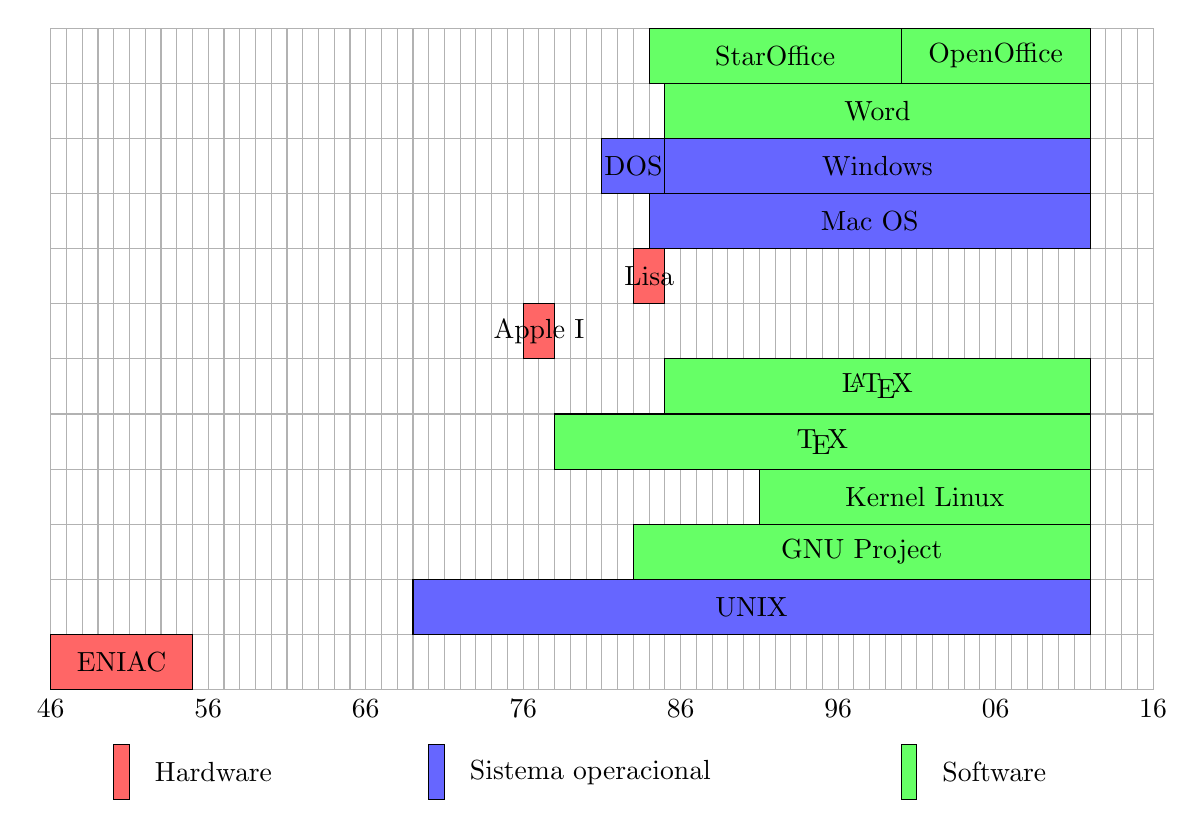
\begin{tikzpicture}[xscale=0.2, yscale=0.7]
    \draw[gray!60] (46,0) grid (116,12);
    \foreach \y in {46, 56, ..., 96}{
        \node[below] at (\y, 0) {\y};
    }
    \node[below] at (106,0) {06};
    \node[below] at (116,0) {16};

    \draw[fill=red!60] (50,-1) rectangle ++(1,-1) ++(1,.5) node[right]{Hardware};
    \draw[fill=blue!60] (70,-1) rectangle ++(1,-1) ++(1,.5) node[right]{Sistema operacional};
    \draw[fill=green!60] (100,-1) rectangle ++(1,-1) ++(1,.5) node[right]{Software};

    \draw[fill=red!60] (46,0) rectangle (55,1) node[midway]{ENIAC};
    \draw[fill=blue!60] (69,1) rectangle (112,2) node[midway]{UNIX};
    \draw[fill=green!60] (83,2) rectangle (112,3) node[midway]{GNU Project};
    \draw[fill=green!60] (91,3) rectangle (112,4) node[midway]{Kernel Linux};
    \draw[fill=green!60] (78,4) rectangle (112,5) node[midway]{\TeX};
    \draw[fill=green!60] (85,5) rectangle (112,6) node[midway]{\LaTeX};
    \draw[fill=red!60] (76,6) rectangle (78,7) node[midway]{Apple I};
    \draw[fill=red!60] (83,7) rectangle (85,8) node[midway]{Lisa};
    \draw[fill=blue!60] (84,8) rectangle (112,9) node[midway]{Mac OS};
    \draw[fill=blue!60] (81,9) rectangle (85,10) node[midway]{DOS};
    \draw[fill=blue!60] (85,9) rectangle (112,10) node[midway]{Windows};
    \draw[fill=green!60] (85,10) rectangle (112,11) node[midway]{Word};
    \draw[fill=green!60] (84,11) rectangle (100,12) node[midway]{StarOffice};
    \draw[fill=green!60] (100,11) rectangle (112,12) node[midway]{OpenOffice};
\end{tikzpicture}

    \end{center}
    \caption{Linha do tempo de alguns softwares.}
    \label{fig:history_timeline}
\end{figure}
